%; whizzy paragraph -pdf xpdf -latex ./whizzypdfptex.sh
%; whizzy-paragraph "^\\\\begin{frame}\\|\\\\emtext"
% latex beamer presentation.
% platex, latex-beamer でコンパイルすることを想定。 

%     Tokyo Debian Meeting resources
%     Copyright (C) 2012 Junichi Uekawa

%     This program is free software; you can redistribute it and/or modify
%     it under the terms of the GNU General Public License as published by
%     the Free Software Foundation; either version 2 of the License, or
%     (at your option) any later version.

%     This program is distributed in the hope that it will be useful,
%     but WITHOUT ANY WARRANTY; without even the implied warreanty of
%     MERCHANTABILITY or FITNESS FOR A PARTICULAR PURPOSE.  See the
%     GNU General Public License for more details.
%     You should have received a copy of the GNU General Public License
%     along with this program; if not, write to the Free Software
%     Foundation, Inc., 51 Franklin St, Fifth Floor, Boston, MA  02110-1301 USA

\documentclass[cjk,dvipdfmx,12pt]{beamer}
\usetheme{Tokyo}
\usepackage{monthlypresentation}

%  preview (shell-command (concat "evince " (replace-regexp-in-string "tex$" "pdf"(buffer-file-name)) "&")) 
%  presentation (shell-command (concat "xpdf -fullscreen " (replace-regexp-in-string "tex$" "pdf"(buffer-file-name)) "&"))
%  presentation (shell-command (concat "evince " (replace-regexp-in-string "tex$" "pdf"(buffer-file-name)) "&"))

%http://www.naney.org/diki/dk/hyperref.html
%日本語EUC系環境の時
\AtBeginDvi{\special{pdf:tounicode EUC-UCS2}}
%シフトJIS系環境の時
%\AtBeginDvi{\special{pdf:tounicode 90ms-RKSJ-UCS2}}

\newenvironment{commandlinesmall}%
{\VerbatimEnvironment
  \begin{Sbox}\begin{minipage}{1.0\hsize}\begin{fontsize}{8}{8} \begin{BVerbatim}}%
{\end{BVerbatim}\end{fontsize}\end{minipage}\end{Sbox}
  \setlength{\fboxsep}{8pt}
% start on a new paragraph

\vspace{6pt}% skip before
\fcolorbox{dancerdarkblue}{dancerlightblue}{\TheSbox}

\vspace{6pt}% skip after
}
%end of commandlinesmall

\title{東京エリアDebian勉強会}
\subtitle{第137回 2016年2月度 OSC 出張勉強会}
\author{岩松 信洋}
\date{2016年2月27日}
\logo{
\includegraphics[width=8cm]{image200607/openlogo-light.eps}}

\begin{document}

\begin{frame}
\titlepage{}
\end{frame}

\begin{frame}{Agenda}
 \begin{minipage}[t]{0.45\hsize}
  \begin{itemize}
   \item 事前課題発表
   \item 最近あったDebian関連のイベント報告
	 \begin{itemize}
	 \item 第135回東京エリアDebian勉強会
	 \end{itemize}
  \end{itemize}
 \end{minipage} 
 \begin{minipage}[t]{0.45\hsize}
  \begin{itemize}
   \item Debian Trivia Quiz
   \item Debian GNU/Linux 上での省電力設定について
   \item libhinawa というライブラリを Debian プロジェクトに ITP/RFS した話
   \item 今日の宴会場所
  \end{itemize}
 \end{minipage}
\end{frame}

\section{事前課題}
\emtext{事前課題}
{\footnotesize
 \begin{prework}{ takaswie }
  \begin{enumerate}
  \item Q.hack time に何をしますか?\\
    A.hinawa-utils の開発。あるいはALSAの開発。\\
https://github.com/takaswie/hinawa-utils
  \item Q.本勉強会をどこでお知りになりましたか?(任意回答)\\
    A. ML
  \end{enumerate}
\end{prework}


\begin{prework}{ mkouhei }
  \begin{enumerate}
  \item Q.hack time に何をしますか?\\
    A.
    \begin{itemize}
    \item https://qa.debian.org/developer.php? login=mkouhei@palmtb.net のメンテ。
    \item パッケージ ( https://qa.debian.org/developer.php? login=mkouhei@palmtb.net ) のメンテナンス
    \item keybase.io を signing-party( caff ) のキーサーバーとして利用できないかの検証

   \end{itemize}
    \item Q.本勉強会をどこでお知りになりましたか?(任意回答)\\
    A. 常連
   \end{enumerate}
\end{prework}

\begin{prework}{ Poeto }
  \begin{enumerate}
  \item Q.hack time に何をしますか?\\
    A.「 Debian 」 の基本操作。( 数日前、インストールしたばかりなので )
  \item Q.本勉強会をどこでお知りになりましたか?(任意回答)\\
    A. Web
  \end{enumerate}
\end{prework}

\begin{prework}{ kenhys }
  \begin{enumerate}
  \item Q.hack time に何をしますか?\\
    A. 未定。
  \item Q.本勉強会をどこでお知りになりましたか?(任意回答)\\
    A. ML
  \end{enumerate}
\end{prework}

\begin{prework}{ iwamatsu }
  \begin{enumerate}
  \item Q.hack time に何をしますか?\\
    A. package メンテナンス。
  \item Q.本勉強会をどこでお知りになりましたか?(任意回答)\\
    A. ML
  \end{enumerate}
\end{prework}

\begin{prework}{ Charies }
  \begin{enumerate}
  \item Q.hack time に何をしますか?\\
    A. パッケージング。
  \end{enumerate}
\end{prework}

\begin{prework}{ dictoss }
  \begin{enumerate}
  \item Q.hack time に何をしますか?\\
    A. kfreebsd の Intel GPU ビデオドライバのデバッグ( unstable で動かなくなった)
  \item Q.本勉強会をどこでお知りになりましたか?(任意回答)\\
    A. Web
  \end{enumerate}
\end{prework}

\begin{prework}{ rosh }
  \begin{enumerate}
  \item Q.hack time に何をしますか?\\
    A. d-i に関する作業
  \item Q.本勉強会をどこでお知りになりましたか?(任意回答)\\
    A. twitter
  \end{enumerate}
\end{prework}

\begin{prework}{ wskoka }
  \begin{enumerate}
  \item Q.hack time に何をしますか?\\
    A. tilegx
  \end{enumerate}
\end{prework}

\begin{prework}{ yy\_y\_ja\_jp }
  \begin{enumerate}
  \item Q.hack time に何をしますか?\\
    A. DDTSS
  \end{enumerate}
\end{prework}

\begin{prework}{ 野島 }
  \begin{enumerate}
  \item Q.hack time に何をしますか?\\
    A. DDTSS、xmrisパッケージ化など。
  \item Q.本勉強会をどこでお知りになりましたか?(任意回答)\\
    A. 幹事なので!\\ところでセミナか、幹事やってみたい人はいつでも募集中!\\貴殿好みの勉強会にしてくれてもよくてよ!
  \end{enumerate}
\end{prework}


}

\section{イベント報告}
\emtext{イベント報告}

\begin{frame}{第135回東京エリアDebian勉強会 }

\begin{itemize}
\item 場所はdotsさんをお借りしての開催でした。
\item 参加者は10名でした。
\item セミナ内容は、2本建てで、
  \begin{enumerate}
  \item 参加者皆さんによる「 Debian 今年の半年分の計画を立ててみた 」
  \item 野島さんによる「 Debian で Linux Ftrace まわりをいじってみた  」
  \end{enumerate}
でした。
\item 残りの時間でhack timeを行い、成果発表をしました。
\end{itemize} 
\end{frame}

\begin{frame}{第135回東京エリアDebian勉強会(つづき)}

  「Debian 今年の半年分の計画を立ててみた」は、2016年6月末までのDebianプロジェクトで行う目標を書いて頂きました。みなさん、がっちり目標を立てていただけました。あとは、実行あるのみということで、よろしくおねがいします!

\end{frame}

\begin{frame}{第135回東京エリアDebian勉強会(つづき)}

  「Debian で Linux Ftrace まわりをいじってみた」は、linux kernelに搭載されているデバッグI/FであるFtraceをDebianで利用してみた事について語られました。Debian sidに搭載されているkernelが4.3.3であることから、USDTを利用してみたり、kprobeを利用した話をしました。Debianに搭載されているFtrace利用のツールである、perf-toolが古かった件についても、BUG Report\footnote{https://bugs.debian.org/813769}が行われました。

\end{frame}

\begin{frame}{第135回東京エリアDebian勉強会(つづき)}

  Debianは、パッケージが古いなどの件もBUG Reportすることでも改善を図ることが出来ます。もし、他に、
\begin{itemize}
\item パッケージが古い、
\item 導入したパッケージのソフトウェアの挙動がおかしい(バグっている)
\item パッケージはこうして欲しい
\end{itemize}
などの要望がありましたら、「誰でも」reportbugツールを使って簡単に改善の要請をすることが出来ます。是非、皆様もどしどしBUG Reportしてくださいませ。
  
\end{frame}

\begin{frame}{第135回東京エリアDebian勉強会(つづき)}

  また、hack timeですが、成果をtitanpad.comに記載する試みを行いました。
以下は前回のhack time中の成果の一覧となります。
\begin{itemize}
\item henrichさん\\
  proposal for Debian idea
  \begin{itemize}
  \item integrate piuparts into repository pipeline
  \item replace dput $\rightarrow$ lintian + piuparts, then upload
   + prevents regression into repository
  \end{itemize}
\item kenhys \\
libhinawaのdebian/*に手をいれていくつかPRを投げたり、issueを立てたりした\\
https://github.com/takaswie/libhinawa/pull/20\\
https://github.com/takaswie/libhinawa/pull/21\\
https://github.com/takaswie/libhinawa/pull/24
\end{itemize}
\end{frame}

\begin{frame}{第135回東京エリアDebian勉強会(つづき)}

\begin{itemize}
\item taiさん\\
  \begin{itemize}
  \item キーサインを行った。 caffではなく手動で\\
    Keysigning with the GNU/Linux Terminal\\
    \url{http://www.phillylinux.org/keys/terminal.html}\\
    に沿ってやってみた。しかし最後の署名したキーを送る所がGmail経由になり署名・暗号化せずに返送してしまったので、caffがやっぱりいいのか・・・
  \item Debian Wikiの翻訳し残しの続きをもくもくと。
  \end{itemize}
\item wskokaさん\\
  tilegx用パッケージ作成(10こぐらい。トータルは1200個ぐらいある。)
\end{itemize}
\end{frame}

\begin{frame}{第135回東京エリアDebian勉強会(つづき)}

\begin{itemize}
\item roshさん\\
  \begin{itemize}
  \item caff でキーサインが出来た\\
  \item 前マージされたLinkstation DTS [0] をベースにて、新Linkstationデバイス (LS-QVL)の DTS を別のユーザ様が出来たとの連絡がありました。今週受け入れられた Linkstation DTS [1] にマージを行いました。これから ARM kernel lists にアップする予定です。\\
    \begin{enumerate}
    \item Kernel tree: arch/arm/boot/dts/kirkwood-{lswvl,lswxl}.dts
    \item \url{http://lists.infradead.org/pipermail/linux-arm-kernel/2016-January/400949.html}
    \end{enumerate}
  \end{itemize}
\end{itemize}
\end{frame}

\begin{frame}{第135回東京エリアDebian勉強会(つづき)}

\begin{itemize}
\item dictossさん \\
  \begin{itemize}
  \item rasberry pi2のdebian jessieからbluetoothテザリングできた
  \item キーサインしました
  \item 東京エリアDebian勉強会のwebサイトをHTML5対応とスマートフォン対応作業(リポジトリの場所確認、ソースコードを読んで中身と作りを把握中)\footnote{2016年2月27日に無事リリースされ、tokyodebian.alioth.debian.orgは、祝!モバイルフレンドリーになりました!}
  \end{itemize}
\item y.yさん
  \begin{itemize}
   \item 参加者とkey signを行った。
   \item Caffで、溜まっていた keysigning 処理のキューをフラッシュできた。
  \end{itemize}
\end{itemize}
\end{frame}

\begin{frame}{第135回東京エリアDebian勉強会(つづき)}

\begin{itemize}
\item takaswieさん\\
 Echo Audio Corp.のFireworksデバイスモジュール向けコマンドラインツールがだいたい書けた。\\
\url{https://github.com/takaswie/hinawa-utils}
\item  yy\_y\_ja\_jpさん\\
  \begin{itemize}
  \item uim-qt5 バグレポート
  \item キーサイン
  \item DDTSS
  \end{itemize}
\item 野島さん
  \begin{itemize}
  \item 9個のDDTSSのレビューを行いました。なお、yorickはtypoの''M-x Yorick''を見落とし、requeueしました。
  \end{itemize}
  
\end{itemize}
\end{frame}

\section{Debian Trivia Quiz}
\emtext{Debian Trivia Quiz}
\begin{frame}{Debian Trivia Quiz}

  Debian の常識、もちろん知ってますよね?
知らないなんて恥ずかしくて、知らないとは言えないあんなことやこんなこと、
みんなで確認してみましょう。

 今回の出題範囲は\url{debian-devel-announce@lists.debian.org},
\url{debian-news@lists.debian.org} に投稿された
内容などからです。

\end{frame}

\subsection{問題}

%; whizzy-master ../debianmeetingresume201311.tex
% $B0J>e$N@_Dj$r$7$F$$$k$?$a!"$3$N%U%!%$%k$G(B M-x whizzytex $B$9$k$H!"(Bwhizzytex$B$,MxMQ$G$-$^$9!#(B
%

\santaku
{2016/2/3$B$K$F!"(Bdebtag$B$N(Btag$BIU$1$K$D$$$F$NJQ99$,N.$l$^$7$?!#0J2<$N$I$l!)(B}
{tag$BIU$1GQ;_(B}
{tag$BIU$1$K$D$$$F%f!<%6G'>ZIU$-$K$9$k(B}
{tag$B$N%l%S%e!<$r$5$i$K6/8G$K$9$k(B}
{B}
{debtag$B$rJT=8$G$-$k%5%$%H$,$$$m$$$m%j%K%e!<%"%k$9$k$H$$$&%"%J%&%s%9$,N.$l!"<B:]$$$/$D$b<B9T$5$l$?$h$&$G$9!#$^$:!"F?L>$K$h$k(Btag$BIU$1$NJT=8$rGQ;_$7!"Be$o$j$K(Bsso.debian.org$B$K$h$k%7%s%0%k%5%$%s%*%s$G%f!<%6G'>Z$7$J$$$HJT=8=PMh$J$$$h$&$K$7$?$H$N$3$H!#$^$?!"(Btag$BJT=8$N(BURL$B$,JQ99$K$J$C$F$*$j!"(Bhttps://debtags.debian.org/$B$H$J$j$^$7$?!#B>$K$b$$$m$$$mJQ99$,=P$F$$$^$9$N$G!">\$7$/$O(Bhttps://lists.debian.org/debian-devel-announce/2016/02/msg00000.html $B;2>H!#(B}

\santaku
{2016/1/12$B$K$F!"(Bdebian sid$B$K(Bphp$B$N?7$7$$%P!<%8%g%s$rF~$l$?7o$,%"%J%&%s%9$5$l$^$7$?!#$I$N%P!<%8%g%s!)(B}
{php 7.0}
{php 5.6}
{php$B$C$F2?!)(B}
{A}
{php7.0$B$,(Bdebian sid$B$K$F%j%j!<%9$5$l$^$7$?!#$A$J$_$K!"(Bphp7$B$NL\6L5!G=$OBgI}$J<B8zB.EY2~A1$G$9!#$3$l$G<!4|0BDjHG%P!<%8%g%s$G$"$k(Bstrech$B$G!"(Bphp7$B$,MxMQ$G$-$k8+9~$_$,$H$F$b9b$/$J$C$F$-$^$7$?$M!*(B}

\santaku
{dbgsym$B%Q%C%1!<%8$G$9$,!"$3$A$i$rJ]4I$9$k%_%i!<@h$O$I$3$G$7$g$&!)(B}
{mirrors.debian.org}
{debug.mirrors.debian.org}
{ftp.jp.debian.org}
{B}
{debhelper 9.20151219$B0J9_$K$F!">o$K%G%P%C%0MQ%7%s%\%k$r<}$a$?%Q%C%1!<%8!JL>A0$O%Q%C%1!<%8L>(B-dbgsym)$B$r@8@.$9$k$h$&$K$J$j$^$7$?!#$3$N(B-dbgsym$B%Q%C%1!<%8$NJ]4I@h$,%"%J%&%s%9$5$l!"(Bhttp://debug.mirrors.debian.org/debian-debug/$B$H!"(Bhttp://snapshot.debian.org/archive/debian-debug/$B$K$J$C$?$h$&$G$9!#(B}



\section{Debian GNU/Linux 上での省電力設定について}
\emtext{Debian GNU/Linux 上での省電力設定について}

\begin{frame}{はじめに}

\begin{itemize}
\item Linux がインストールされたノートPCを利用している時、スペック通りにバッテリが持たない
\item デフォルトの設定では省電力設定ができていない。
\item デフォルトの設定ではなく、パラーメータを調整して、よりよいノートPC生活を送りたい
\item Debian GNU/Linux での省電力設定を解説
\end{itemize}

\end{frame}

\begin{frame}{省電力設定するためには}

\begin{itemize}
\item CPUと制御
\item 動作しているデバイス
\item 動作しているプログラム
\end{itemize}
\end{frame}

\begin{frame}{CPUと制御}

\begin{figure}[H]
\begin{center}
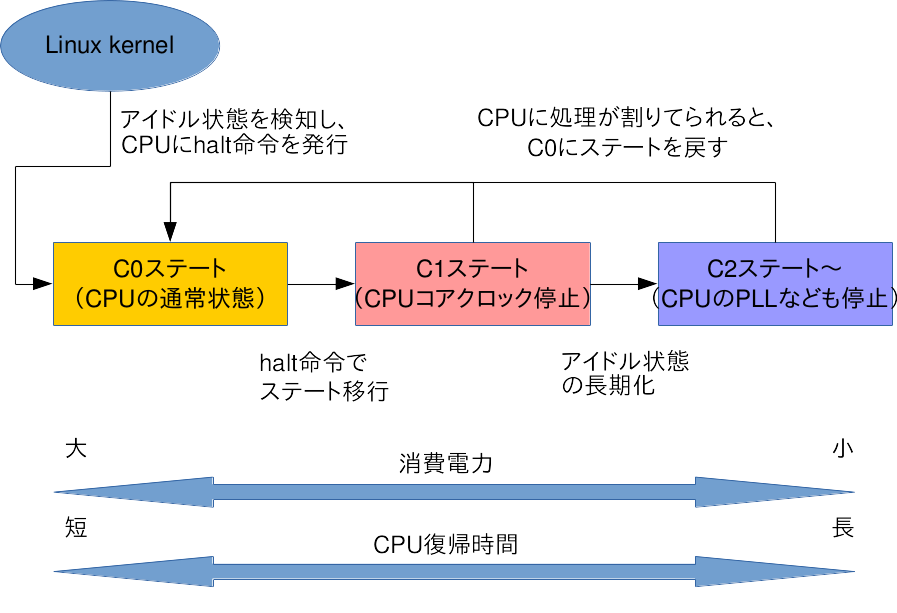
\includegraphics[width=0.8\hsize]{image201602/cpustate.png}
\end{center}
\label{fig:cpustate}
\caption{CPU状態遷移簡易図} 
\end{figure}

\end{frame}

\begin{frame}[containsverbatim]{CPU周波数スケーリング機能とcpufreq-info}

Linux の場合はCPU周波数スケーリング機能があり、cpufreq 機構として
実装されている。

\begin{figure}[htbp]
\begin{commandline}
$ cpufreq-info
cpufrequtils 008: cpufreq-info (C) Dominik Brodowski 2004-2009
Report errors and bugs to cpufreq@vger.kernel.org, please.
analyzing CPU 0:
  driver: intel_pstate
  CPUs which run at the same hardware frequency: 0
  CPUs which need to have their frequency coordinated by software: 0
  maximum transition latency: 0.97 ms.
  hardware limits: 800 MHz - 2.90 GHz
  available cpufreq governors: performance, powersave
  current policy: frequency should be within 800 MHz and 2.90 GHz.
                  The governor "powersave" may decide which speed to use
                  within this range.
  current CPU frequency is 1.90 GHz.
....
\end{commandline}
\caption{cpufreq-info 実行結果}
\label{fig:cpufreq-info}
\end{figure}

\end{frame}

\begin{frame}{ガバナーと現在設定されているポリシー}

\begin{table}[htb]
\begin{center}
\begin{tabular}{l|l}
ガバナー & 内容 \\
ondemand &	CPU負荷が大きい、または小さい時に \\
         &      CPUクロックを大きくに切り替える \\
conservative &	CPU負荷が大きい、または小さい時に\\
	     &  CPUクロックを徐々に切り替える \\
performance &	最大周波数でCPUを動作させる \\
powersave &	最小周波数でCPUを動作させる \\
userspace &	ユーザーが指定した周波数でCPUを動作させる \\
\end{tabular}
\caption{指定できるガバナー}
\label{tab:governors}
\end{center}
\end{table}

\end{frame}

\begin{frame}[containsverbatim]

\begin{itemize}
\item CPUが800MHzから2.90GHzまでをサポートしている
\item powersave governor で動作している
\item 最大値と最小値のポリシー設定により、800MHzから2.90GHzの間で変動させている
\end{itemize}

\begin{commandline}
$ cpufreq-info
cpufrequtils 008: cpufreq-info (C) Dominik Brodowski 2004-2009
Report errors and bugs to cpufreq@vger.kernel.org, please.
analyzing CPU 0:
  driver: intel_pstate
  CPUs which run at the same hardware frequency: 0
  CPUs which need to have their frequency coordinated by software: 0
  maximum transition latency: 0.97 ms.
  hardware limits: 800 MHz - 2.90 GHz
  available cpufreq governors: performance, powersave
  current policy: frequency should be within 800 MHz and 2.90 GHz.
                  The governor "powersave" may decide which speed to use
                  within this range.
  current CPU frequency is 1.90 GHz.
....
\end{commandline}

\end{frame}

\begin{frame}[containsverbatim]{ガバナーとCPUクロックの設定}
設定には cpufreq-set コマンドを使う。

ガバナーを設定する
\begin{commandline}
$ sudo cpufreq-set -c CPU番号 -g ガバナー名
または
$ sudo sh -c "echo ガバナー名 > \
  /sys/devices/system/cpu/cpuCPU番号/cpufreq/scaling_governor"
\end{commandline}

\end{frame}

\begin{frame}[containsverbatim]{ガバナーとCPUクロックの設定}

最小クロックを設定する
\begin{commandline}
$ sudo cpufreq-set -c CPU番号 -d クロック値
または
$ sudo sh -c "echo クロック値 > \
  /sys/devices/system/cpu/cpuCPU番号/cpufreq/scaling_min_freq"
\end{commandline}

\end{frame}

\begin{frame}[containsverbatim]{ガバナーとCPUクロックの設定}
最大クロックを設定する
\begin{commandline}
$ sudo cpufreq-set -c CPU番号 -u クロック値
または
$ sudo sh -c "echo クロック値 > \
  /sys/devices/system/cpu/cpuCPU番号/cpufreq/scaling_max_freq"
\end{commandline}

\end{frame}

\begin{frame}[containsverbatim]{ガバナーとCPUクロックの設定}
現在のクロックを設定する
\begin{commandline}
$ sudo cpufreq-set -c CPU番号 -f クロック値
または
$ sudo sh -c "echo クロック値 > \
  /sys/devices/system/cpu/cpuCPU番号/cpufreq/scaling_cur_freq"
\end{commandline}

\end{frame}

\begin{frame}{ガバナーとCPUクロックの設定}

\begin{itemize}
\item sysfs を使った設定は再起動すると消えてしまう。
\item /etc/sysfs.conf を使うか、cpufreqd パッケージで設定できるようにする。
\end{itemize}

\end{frame}

\begin{frame}{動作しているデバイスの設定}

\begin{itemize}
\item 使わないデバイスを有効にするだけで電力を消費する。
\item 環境に応じてデバイスの電力等を制御する。
\item ここではよく利用されるデバイスに対する制御方法について紹介。
\end{itemize}

\end{frame}

\begin{frame}[containsverbatim]{ラップトップモード}

ラップトップモード設定
\begin{commandline}
$ sudo sh -c "echo 5 > /proc/sys/vm/laptop_mode"
\end{commandline}

NMI watchdog 無効化
\begin{commandline}
$ sudo sh -c "echo 0 > /proc/sys/kernel/nmi_watchdog"
\end{commandline}

\end{frame}

\begin{frame}[containsverbatim]{USB}
USB は /sys/bus/usb/devices/ 以下に対して設定。

\begin{commandline}
$ sudo sh -c "echo off > \
  /sys/bus/usb/devices/usb1/power/control"
$ sudo sh -c "echo auto > \
  /sys/bus/usb/devices/usb1/power/autosuspend"
\end{commandline}

起動時に再設定したい場合は udev の rules ファイルを用意する。

\begin{commandline}
$ cat /etc/udev/rules.d/70-my-usb-power.rules
ACTION=="add", SUBSYSTEM=="usb", ATTRS{idVendor}=="0x046d", \
      ATTR{idProduct}=="0x08cb", TEST=="power/control", \
      ATTR{power/control}="off"
\end{commandline}

\end{frame}

%注意しなければいけない点としてはUSBをなんでも設定してしまうとキーボードが動作しなくなる可能性もあるため、
%ベンダーID、デバイスIDなどを確認した上で設定しましょう。

\begin{frame}[containsverbatim]{無線LAN}

無線LANは iw パッケージに含まれる iw コマンドを使って設定する。

\begin{commandline}
$ sudo iw dev wlan0 set power_save on
\end{commandline}

udev の rules ファイルを使って設定方法

\begin{commandline}
$ cat /etc/udev/rules.d/70-my-wifi-power.rules
ACTION=="add", SUBSYSTEM=="net", KERNEL=="wlan*", \
      RUN+="/usr/bin/iw dev %k set power_save on"
\end{commandline}

\end{frame}

\begin{frame}[containsverbatim]{サウンド}

\begin{commandline}
$ sudo sh -c "echo 1 > \
  /sys/module/snd_hda_intel/parameters/power_save"
\end{commandline}

\end{frame}

\begin{frame}[containsverbatim]{PCI/PCI-Express}
PCI/PCI-Express の省電力に設定するには power/control を auto に設定する。

\begin{commandline}
$ sudo sh -c "echo auto > \
  /sys/bus/pci/devices/0000:00:00.0/power/control"
\end{commandline}

\end{frame}

\begin{frame}{動作しているプログラムについて}

\begin{itemize}
\item top コマンドである程度わかるが、細かい数字はわからない。
\item PowerTOP を使って確認する。
\end{itemize}

\end{frame}

\begin{frame}{省電力設定するためのツール}

\begin{itemize}
\item 省電力設定するには専門の知識が必要。
\item 細々とした設定をひとつづつやっていくのは大変。
\item 専門知識がなくても、ざっくりとやってくれるツールがある。
\item これらのツールを紹介
\end{itemize}

\end{frame}

\begin{frame}{PowerTOP}

\begin{itemize}
\item Intelが開発しているソフトウェア。
\item Linux カーネル、ハードウェア、ユーザランドで制御可能な省電力項目を
有効にするツール。
\item プロセスを監視して、CPU負荷やデバイスドライバの使用状況のレポートなどが行える
\end{itemize}

\end{frame}

\begin{frame}[containsverbatim]{インストール}

\begin{commandline}
% sudo apt-get install powertop	
\end{commandline}

\end{frame}

\begin{frame}[containsverbatim]{起動}

\begin{figure}[H]
\begin{center}
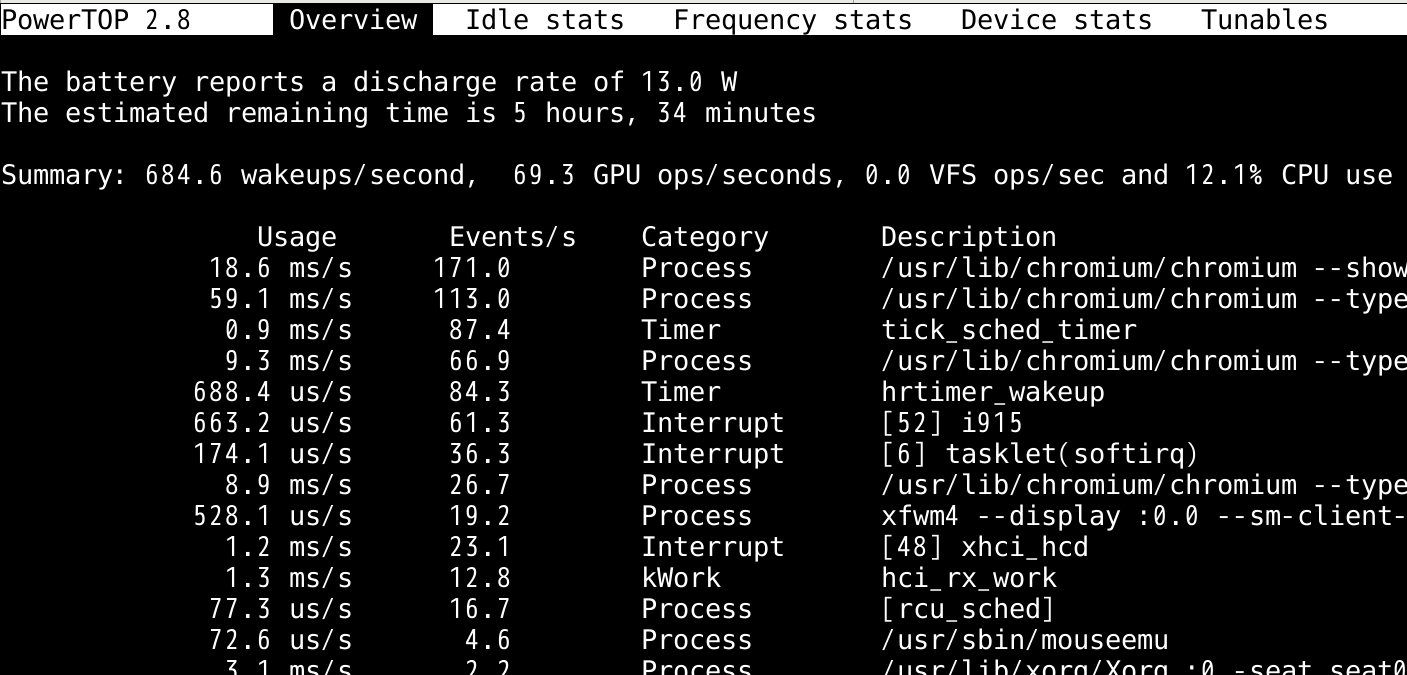
\includegraphics[width=0.8\hsize]{image201602/powertop_00.png}
\end{center}
\label{fig:powertop0}
\caption{PowerTOP起動画面} 
\end{figure}

\end{frame}

\begin{frame}[containsverbatim]{Tunables タブ}
\begin{itemize}
\item Tunables タブには調整可能なシステムの設定が表示される。
\item Badが省電力に有効な項目にもかかわらず無効な設定。
\item Good が既に有効になっている設定。
\end{itemize}

\begin{figure}[H]
\begin{center}
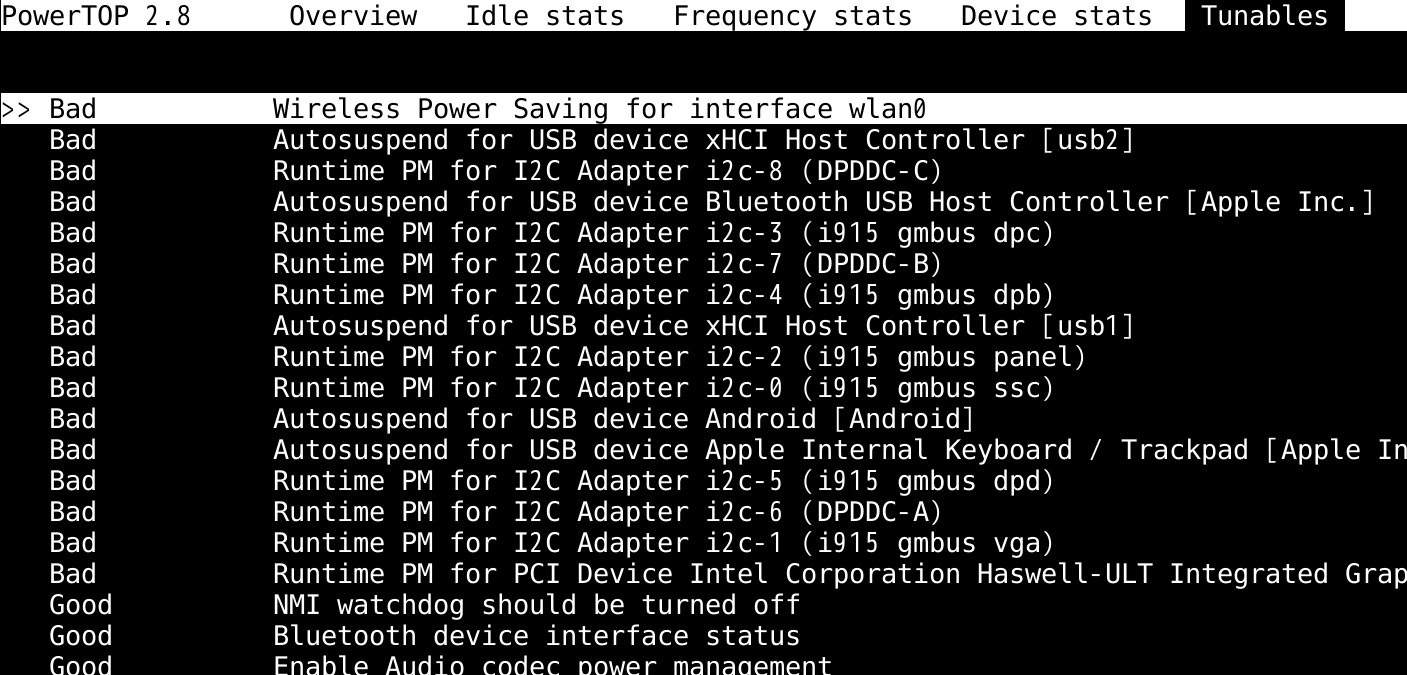
\includegraphics[width=0.8\hsize]{image201602/powertop_01.png}
\end{center}
\label{fig:powertop1}
\caption{Tunables画面} 
\end{figure}

この状態ではまだシステムに最適化された設定になっていないため、一度終了し、
キャリブレーションを行う。

\end{frame}

\begin{frame}[containsverbatim]{キャリブレーション}

実行するとデバイスなどから使用状況を読み取り、マシンに対して適切な設定を
行う。
ノートPCの場合はいきなりモニターのバックライトが消えるので注意。

\begin{commandline}
$ sudo powertop --calibrate
\end{commandline}

\end{frame}

\begin{frame}[containsverbatim]{キャリブレーション}

\begin{itemize}
\item キャリブレーションが終わると、\texttt{/var/cache/powertop/saved\_parameters.powertop}
以下にデータが保存される。
\item 次回のPowerTOP起動時からはキャリブレーションデータを元に
省電力にされた環境で起動する。
\end{itemize}

\end{frame}

\begin{frame}[containsverbatim]{キャリブレーション後}

キャリブレーション後に起動すると、
「The battery reports a discharge rate ...」 の項目に表示される消費電力値が変わり、システム
全体で省電力で稼働している事が確認できるはず。

\end{frame}

\begin{frame}[containsverbatim]{PowerTOP の起動時有効化}

\begin{itemize}
\item PowerTOP は起動すると保存されている設定を元に省電力状態にしてくれますが、PCを立ち上げるたびに
PowerTOP自体を立ち上げる必要がある。
。

\item 起動時に自動的にPowerTOP を立ち上げるようにするには、以下のように systemd の ユニットファイル
を用意し、有効にする。

\begin{commandline}
$ cat /etc/systemd/system/powertop.service

[Unit]
Description=PowerTOP

[Service]
Type=oneshot
ExecStart=/usr/bin/powertop
Environment="TERM=xterm"

[Install]
WantedBy=multi-user.target
\end{commandline}

\begin{commandline}
$ sudo systemctl enable powertop
\end{commandline}

\end{itemize}

\end{frame}

\begin{frame}[containsverbatim]{TLP を使った設定}

\begin{itemize}
\item PowerTOPのように詳細なレポートは
出さないが、AC接続時などの状況に応じたスクリプトが準備されており、インストール
するだけである程度省電力設定を行ってくれる便利なツール。
\item Debian ではパッケージ化されており、apt でインストールできる。
\begin{commandline}
$ sudo apt-get install tlp
\end{commandline}

\end{itemize}

\end{frame}


\begin{frame}[containsverbatim]{TLP を使った設定}

\begin{itemize}
\item 無線LANの設定等に NetworkManager を使っているなら tlp-rdw パッケージもインストールしておくと
無線LAN、Bluetooth関連の設定も行ってくれる。

\item デフォルトの設定は /etc/default/tlp にあり、このファイルを変更して環境に合わせた省電力設定を
行う。

\end{itemize}
\end{frame}

\begin{frame}[containsverbatim]{TLP を使った設定}
\begin{itemize}

\item 設定はよく使われる項目しかなく、使っている環境の設定がない場合もある。このような場合は
自分で設定を追加するか、先に説明したようにsysfs / procfs 経由
の設定を別途行う必要がある。

\begin{center}
\begin{commandline}
# Set to 0 to disable, 1 to enable TLP.
TLP_ENABLE=1

# Operation mode when no power supply can be detected: AC, BAT
# Concerns some desktop and embedded hardware only.
TLP_DEFAULT_MODE=AC

# Seconds laptop mode has to wait after the disk goes idle before doing a sync.
# Non-zero value enables, zero disables laptop mode.
DISK_IDLE_SECS_ON_AC=0
DISK_IDLE_SECS_ON_BAT=2

# Dirty page values (timeouts in secs).
MAX_LOST_WORK_SECS_ON_AC=15
MAX_LOST_WORK_SECS_ON_BAT=60
...
\end{commandline}
\end{center}

TLP は systemd やその他init用の起動ファイルが用意されているのでPC起動時に設定が反映されるのも
良い点です。

\end{itemize}

\end{frame}

\begin{frame}{省電力設定後}
\begin{itemize}
\item 省電力設定した後に PowerTOP で消費電力を確認。
\item 消費電力が13W から 11W に下がっている。
\item PC稼働時間も5時間半から6時間50分に伸びている
\end{itemize}

\begin{figure}[H]
\begin{center}
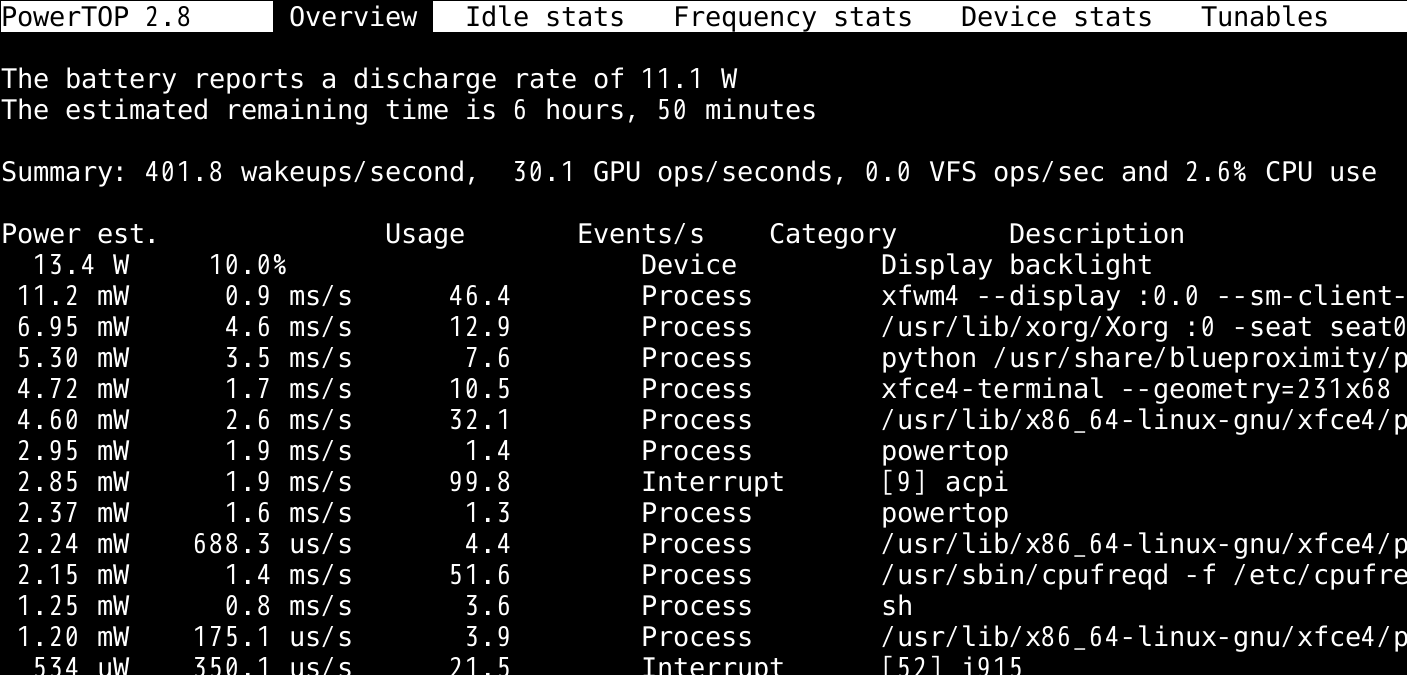
\includegraphics[width=0.8\hsize]{image201602/powertop_02.png}
\end{center}
\label{fig:powertop2}
\caption{省電力設定後} 
\end{figure}

\end{frame}

\begin{frame}{まとめ}

\begin{itemize}

\item Debian GNU/Linuxでの省電力設定について説明した。
\item 現在の状態をとりあえず確認するには cpufreq-info を使い、カーネルの設定やドライバの設定は
sysfs や proc fs 経由で設定する。
\item プログラムやプロセスの詳細な状態の確認するには
PowerTOPを使う。省電力設定できる項目もわかり、ユーザインターフェイスから各種設定ができるようになっている。
%\item PCを再立ち上げすると PowerTOP を起動させる必要があるた、sysytem用のserviceファイルを別途用意するなどの対策が必要です。
\item
細かい設定を行わなくても、とりあえず省電力設定を行いたい場合はTLPを使うのがよい。ただ全てのPCをサポートしているわけではないので、環境に合わせてプログラムを修正するなりの対応が必要となる。
\item 細かい設定をしたい場合は sysfs や procfsから設定する必要がある。この場合専門の知識が必要となる。

\end{itemize}
\end{frame}


\section{libhinawa というライブラリを Debian プロジェクトに ITP/RFS した話}
\emtext{libhinawa というライブラリを Debian プロジェクトに ITP/RFS した話}

\begin{frame}{概要}
  libhinawaというライブラリをDebianプロジェクトにITP/RFSしたので、
  その背景や設計、機能に関して、ALSAのupstreamでの活動も踏まえて
  お話します。
\end{frame}

\begin{frame}{内容}
  \begin{itemize}
  \item ALSAについて
  \item libhinawaについて
  \item 今回のITP/RFSについて
  \end{itemize}
  質疑は適宜行ってください。
\end{frame}

\begin{frame}{ALSAの概要}
  ALSA
  \begin{itemize}
  \item Linux sound subsystem
  \item ユーザースペースのアプリケーションに対し、サウンドデバイスを
        制御する手段を提供
  \item 特定のサウンドデバイスに対しては、CUIやGUIを伴うツールを提供
  \end{itemize}
  ALSAを利用しているもの
  \begin{itemize}
  \item Linuxカーネルを採用した製品全般
  \end{itemize}
\end{frame}

\begin{frame}{ALSAがサポートするサウンドデバイス}
  \begin{itemize}
  \item PCI/PCI-Expressバスに接続するもの
  \item プラットフォーム固有のペリフェラルバスに接続するもの
  \item USBに接続するもの
  \item 他、レガシーな汎用バスに接続するもの (IEEE 1394バス)
  \end{itemize}
\end{frame}

\begin{frame}{ALSAとIEEE 1394バス}
  2000-2010年にかけて、IEEE 1394バスに接続して使う
  サウンドデバイスが発売されていた。
  \begin{itemize}
  \item 主にレコーディング用途
  \item 一部の高級オーディオ機器
  \end{itemize}
  ALSAでのサポートは2010年に始まった。
  \begin{itemize}
  \item Linux 2.6.39に初期のコードをマージ
  \item 以降の開発は進まず
  \end{itemize}
\end{frame}

\begin{frame}{ユーザースペースのドライバ実装}
  Linux FireWire subsystemが、キャラクタデバイス越しに
  デバイスを制御する手段をユーザースペースに提供
  \begin{itemize}
  \item /dev/fw[0-9]*
  \end{itemize}
  FFADO
  \begin{itemize}
  \item ユーザースペースのドライバ開発プロジェクト
  \item \url{http://ffado.org/}
  \item libffado2として、CのライブラリAPIを公開
  \item 2004年あたりに開発開始
  \end{itemize}
  ALSAとは異なるAPI
  \begin{itemize}
  \item ALSAのアプリケーションから使えない
  \item プロトコル仕様(IEC 61883-1/6)的に、ALSA-FFADO
        ブリッジが成立しない。
  \end{itemize}
\end{frame}

\begin{frame}{ALSAのfirewireスタックの成長}
  2013年1月時点。2モデルをサポート。
  \begin{itemize}
  \item 2,600行程度
  \end{itemize}
  2016年2月現在、約140モデルをサポートするに至る。
  \begin{itemize}
  \item 20,000行程度
  \end{itemize}
\end{frame}

\begin{frame}{libhinawaの概要}
  ALSAのfirewireスタックの設計
  \begin{itemize}
  \item リアルタイムデータ転送以外の機能はユーザースペースに置く
  \item どうしてもカーネルランドに必要な機能はALSAのHwDepを使って
        ユーザースペースからアクセス可能にする
  \end{itemize}
  当初はFFADOの資産を再利用するつもりだった
  \begin{itemize}
  \item が、それは困難を伴うことが後に判明
  \end{itemize}
\end{frame}

\begin{frame}{FFADOの困難}
  FFADOのツールを開発に用立てるのはむつかしい
  \begin{itemize}
  \item libffado2の設計上の欠陥
  \end{itemize}
  FFADOのコードベースの古さ
  \begin{itemize}
  \item FFADOのツールがPython2で書かれている
  \end{itemize}
  開発に用立てるツールの必要
  \begin{itemize}
  \item libhinawaの開発に着手
  \end{itemize}
\end{frame}

\begin{frame}{libhinawaの設計}
  キャラクタデバイスに対する入出力の抽象
  \begin{itemize}
  \item /dev/fw[0-9]*
  \item /dev/snd/hwC[0-9]*D0
  \end{itemize}
  GObject Introspectionによる、言語バインディングからの利用
  \begin{itemize}
  \item 140デバイスそれぞれ固有の操作が必要
  \item デバイス操作方法を見出す試行錯誤が必要
  \item LLで書きたかった
  \end{itemize}
\end{frame}

\begin{frame}{libhinawaの開発}
  \begin{itemize}
  \item 2014年9月あたりに開発着手。CのライブラリAPIを公開 (0.2.0)
  % [alsa-devel] [RFC] libhinawa: a light-weight I/O library for
status/transactions to ALSA FireWire devices
  %
\url{http://mailman.alsa-project.org/pipermail/alsa-devel/2014-September/081732.html}
  \item 2015年1月にGObject Introspection対応 (0.3.0)
  % [alsa-devel] [RFC] libhinawa: gobject introspection library for
ALSA/FireWire transaction
  %
\url{http://mailman.alsa-project.org/pipermail/alsa-devel/2015-January/086371.html}
  \item その2週間後にalsa-tools.gitに対するRFC (0.4.0)
  % [alsa-devel] [RFC][PATCH 00/13] alsa-tools: libhinawa for control
applications of FireWire devices
  %
\url{http://mailman.alsa-project.org/pipermail/alsa-devel/2015-January/086969.html}
  \item 2015年2月にalsa-libへの依存を破棄 (0.5.0)
  \end{itemize}
\end{frame}

\begin{frame}{libhinawaの開発(つづき)}
  \begin{itemize}
  \item 2015年3月に初期のdebian/rpmパッケージングとそれに伴う修正 (0.6.0)
  \item 2016年1月にDebianへのITPとそれに伴う修正 (0.7.0)
  %[alsa-devel] About planning of libhinawa ITP to debian project
  %
\url{http://mailman.alsa-project.org/pipermail/alsa-devel/2016-February/103771.html}
  \end{itemize}
\end{frame}

\begin{frame}{libhinawa開発の裏}
  メインラインの作業
  \begin{itemize}
  \item Linux 3.16 - 63パッチ
  %\item https://lkml.org/lkml/2014/6/4/895
  \item Linux 3.19 - 31パッチ
  %\item https://lkml.org/lkml/2014/12/11/226
  \item Linux 4.2 - 22パッチ
  %\item https://lkml.org/lkml/2015/6/25/59
  \item Linux 4.4 - 68パッチ
  %\item https://lkml.org/lkml/2015/11/6/410
  \end{itemize}
  Linux stable kernel
  \begin{itemize}
  \item バグが報告されたら、その修正パッチを作ってstableに送る。
  \end{itemize}
\end{frame}

\begin{frame}{libhinawaのITP/RFS}
  作業はgithubを使って進める。
  \begin{itemize}
  \item \url{https://github.com/takaswie/libhinawa/}
  \end{itemize}
  1/14あたり
  \begin{itemize}
  \item 林さんと、libhinawaのITPの話をする。
  \end{itemize}
  1/18
  \begin{itemize}
  \item 林さんから最初のPR
  \end{itemize}
  1/24あたり
  \begin{itemize}
  \item Ubuntu 16.04のDebianImportFreeze(2/17)に間に合わせる方針
  % https://wiki.ubuntu.com/XenialXerus/ReleaseSchedule
  \end{itemize}
  1/28あたり
  \begin{itemize}
  \item Autotools周りの修正終了
  \item debian/* の用意終了
  \end{itemize}
\end{frame}
\begin{frame}{libhinawaのITP/RFS(つづき)}
  1/31
  \begin{itemize}
  \item DebianプロジェクトにITPすることを、Linux FireWire subsystem,
        Linux sound subsystem、FFADOに対して連絡。
  \item
\url{http://mailman.alsa-project.org/pipermail/alsa-devel/2016-January/103693.html}
  \end{itemize}
  2/2
  \begin{itemize}
  \item ITP
  \begin{itemize}
  \item \url{https://bugs.debian.org/cgi-bin/bugreport.cgi?bug=813474}
  \end{itemize}
  \item RFS
  \begin{itemize}
  \item \url{https://bugs.debian.org/cgi-bin/bugreport.cgi?bug=813489}
  \end{itemize}
  \end{itemize}
\end{frame}

\begin{frame}{DebianへのITP/RFS後}
  2/6
  \begin{itemize}
  \item 樋口大輔さんにスポンサードしてもらう
  \item New queue入りする
  \end{itemize}
  2/7
  \begin{itemize}
  \item 朝、ftp-master入り。unstableリポジトリに入る
  \begin{itemize}
  \item \url{https://packages.debian.org/source/sid/libhinawa}
  \end{itemize}
  \item 夜、UbuntuのDebian AutoSync botが捕捉。universeリポジトリに入る。
  \begin{itemize}
  \item \url{https://launchpad.net/ubuntu/+source/libhinawa}
  \end{itemize}
  \item 深夜、アップストリームに報告
  \begin{itemize}
  \item
\url{http://mailman.alsa-project.org/pipermail/alsa-devel/2016-February/104046.html}
  \end{itemize}
  \end{itemize}
\end{frame}

\begin{frame}{まとめ}
\begin{itemize}
\item libhinawaをDebianプロジェクトにITPしました
\end{itemize}
\end{frame}

\section{Hack time}
\emtext{Hack time}

\begin{frame}{成果を記入下さい!}

  今回、Hack time時の成果を記録に残してみます。

\url{https://debianmeeting.titanpad.com/8}

に皆さんアクセス頂き(認証不要です)、各自成果を18:40までに記録するようにおねがいします。

\end{frame}
  
\section{今後のイベント}
\emtext{今後のイベント}
\begin{frame}{今後のイベント}
\begin{itemize}
\item 2/16 Debian developer来日迎撃GPG Beer Signing(2016/2)
 Debianにて、LXDEのパッケージメンテナをされているAndrew Leeさんが来日され、henrichさんにて、飲み会しながらのキーサイン会が行われます。掲示:\url{http://debianjp.connpass.com/event/26965/}
\item 関西エリアDebian勉強会。
\end{itemize}
\end{frame}

\begin{frame}{今後のイベント}
\begin{itemize}
\item 3/5 (土) 第137回東京エリアDebian勉強会\\
  場所はサイボウズ株式会社さんにて!この日、henrichさんのお手配により、ドイツから公式Debian DeveloperのJohn Paul Adrian Glaubitzさんが合流されます!海外 DeveloperのKey Signのチャンス、海外のアクティブなDebian Developerの方とぶっちゃけトークなど出来る貴重なチャンス!さあ、そこの貴方も参加するのだ。
\end{itemize}
\end{frame}

\begin{frame}{今後のイベント(つづき)}
\begin{itemize}
\item 参考:Andrew Leeさんの活動\\
   \url{https://qa.debian.org/developer.php?login=ajqlee}\\
    主にLXDE デスクトップ環境のパッケージなど。
\item 参考:John Paul Adrian Glaubitzさんの活動
  \begin{itemize}
  \item 詳しくは、\url{https://qa.debian.org/developer.php?login=glaubitz\%40physik.fu-berlin.de} DebianのMATE デスクトップ環境の多数のパッケージ群など。
  \item m68k/sh4/sparc64移植作業
  \end{itemize}
\end{itemize}
\end{frame}

\section{今日の宴会場所}
\emtext{今日の宴会場所}
\begin{frame}{今日の宴会場所}
未定
\end{frame}

\end{document}

;;; Local Variables: ***
;;; outline-regexp: "\\([ 	]*\\\\\\(documentstyle\\|documentclass\\|emtext\\|section\\|begin{frame}\\)\\*?[ 	]*[[{]\\|[]+\\)" ***
;;; End: ***
